

\chapter{ Capítulo introductorio}

\begin{chapquote}{Javier, \textit{Todos los días}}
`` Me cago en Dios''
\end{chapquote}

\section{La visión como herramienta}


El ser humano es capaz de interactuar con el mundo que le rodea de diversas maneras ya sean creativas o incluso productivas. Esto se hace con el uso de los sentidos; Tacto, gusto, oído, olfato y por último pero no menos importante la visión. Este sentido nos permite recoger gran cantidad de información del mundo que nos rodea, procesarla y actuar en consecuencia.Es entonces el ojo humano una herramienta de gran valor y elevada precisión que poco tiene que envidiar al órgano semejante en el resto de especies en todo el reino animal. 
Lejos de realizar un estudio anatómico del sentido de la vista en el ser humano, se disponen a continuación ciertas características de interés que permiten apreciar toda su potencia.

Una de las primeras cuestiones que se vienen a la mente cuando se habla de la "simple vista" es su resolución, es decir, cuál es la mínima distancia que es capaz de distinguir. se puede estudiar mediante la resolución angular que para el ser humano se encuentra entorno a 1' o 2' o l que es lo mismo un intervalo de 0,02º a 0,03º. Dicho de otra forma, un ojo humano sano y correctamente desarrollado puede distinguir objetos de entre 30cm y 60cm a 1km de distancia. Por ejemplo, El ojo humano podría servir para detectar dos balones de playa de un diámetro aproximado de 45cm hasta 1km de distancia como máximo. 
Otra manera de comprender la potencia de esta resolución sería posible equiparándola con la potencia de una cámara digital, para el caso, varios cientos de megapíxeles. Véase como ejemplo una cámara Canon de 50,6 Megapíxeles disponible a más de 3500 euros
\textit{comparar vision humana y MPixeles}


El campo de visión es también un aspecto de gran importancia ya que determina la cantidad de información que los ojos pueden recibir en un instante dado. El "cono de visión" queda entorno a unos 130º en vertical y 160º en horizontal
%https://en.wikipedia.org/wiki/Angle_of_view#Common_lens_angles_of_view


Por último, se considera la velocidad de enfoque o acomodación del ojo humano
%http://www.sophimania.pe/ciencia/cerebro-y-neurociencias/estudio-revela-que-el-ojo-humano-capta-una-imagen-en-13-milisegundos/


%https://es.wikipedia.org/wiki/Simple_vista

Se ha planteado entonces una situación en la que hay un pequeño problema, un instrumento de gran precisión y prolongada durabilidad embarcado en un ser vivo falible y en ocasiones errático. No sólo esto sino que nunca se llega a dominar por completo el manejo de éste órgano así como su uso en conjunto a las demás partes del cuerpo y siempre todo ello limitado por la velocidad de respuesta que puede proporcionar el sistema nervioso.
Por ejemplo, ...
%https://www.fuerzaycontrol.com/la-velocidad-de-reaccion-el-tiempo-de-reaccion-simple-complejo-la-anticipacion/

Teniendo en cuenta una posible definición de tecnología 

"La aplicación de conocimientos científicos para la resolución de problemas mediante el diseño y creación de bienes y servicios" 

junto a su etimología, pues se trata de una palabra de origen griego 
%τεχνολογία 
formada por 
%τέχνη 
(arte, técnica u oficio) y 
%λογία 
(el estudio de algo) es fácil apreciar que la evolución y desarrollo del ser humano durante toda su historia han venido ligadas a un progreso tecnológico incesante, vivo y capaz de abrirse paso incluso en las épocas más oscuras de la historia de la humanidad. 
\textit{linea temporal tecnología}
%https://tecnomagazine.net/2018/04/30/historia-de-la-tecnologia/
\\
Una vez descritas brevemente la potencia, capacidad y posibilidades que aporta la visión en el ser humano, se puede ir más allá, subir un nivel y dotar a entes ajenos al hombre de la capacidad de obtener y procesar información visual. Este concepto existe desde finales de la década de los sesenta y puede introducirse como visión artificial o visión por computador: 
\\
“Disciplina científica que incluye métodos para adquirir, procesar, analizar y comprender las imágenes del mundo real con el fin de producir información numérica o simbólica para que puedan ser tratados por un computador”
\\
Esta forma de trabajar con información visual es posible debido a la puesta en conjunto de diferentes campos como la geometría, física o estadística y demás herramientas que se explicarán más adelante.
%https://es.wikipedia.org/wiki/Visi%C3%B3n_artificial#Detecci%C3%B3n_de_objetos


Bien es cierto que se plantea un problema ya que la forma en que el ojo humano percibe el mundo no es la misma en la que lo hace una máquina pues se pueden establecer sus diferencias como las mismas que hay entre una señal analógica y otra digital, respectivamente.
\\
Véase en primer lugar la mencionada diferencia respecto a las señales:

\begin{list}{•}
\item Señal analógica

Se trata de la representación de una magnitud física tal y como se percibe del entorno o se genera con algún instrumento y puede verse como una función matemática continua.
La mayoría de las señales que se perciben son analógicas como ejemplo la intensidad de corriente eléctrica, la temperatura, el sonido, presión y energía.
De este modo existen señales analógicas periódicas (caracterizadas por amplitud y frecuencia) no periódicas (toman cualquier valor independientemente del tiempo)
\textit {ejemplo de señales matlab automatica}

\item Señal digital
\\
Existe una extendida confusión en lo referente a la diferencia entre señal digital y señal discretizada. Se parte de la siguiente señal analógica y sus características en amplitud y frecuencia:
\\
A partir de la señal anterior se llega a una señal discretizada tomando valores equidistantes en el tiempo:
\\
Se llega entonces a una señal digital codificando cada uno de los valores discretos de la señal representada anteriormente. De este modo se tiene un número determinado de valores fijos pertenecientes a un conjunto y no intervalos.

Se puede mostrar el funcionamiento básico de un convertidor Analógico/digital para comprender la diferencia entre estos dos conceptos:
\textit{apuntes micros convertidor y diagrama}

Llevando este concepto al campo de los sistemas digitales, tal y como puede ser un ordenador, se llega al uso de la lógica de dos estados o binaria en la cual existen los estados alto H o 1 y bajo L o 0 en el caso de lógica positiva y H o 0 junto a L o 1 para la lógica negativa.
Un ejemplo de señal digital para la lógica de dos estados:

\textit{señal digital}

A pesar de parecer señales discontinuas, en realidad existen transiciones continuas de un estado a otro llamadas flancos de subida o bajada. 
Se puede apreciar a continuación la misma señal que se ha mostrado en el ejemplo anterior pero en este caso a una escala diferente para poder apreciar la mencionada transición.

\textit{señal digital a escala mayor}
\end{list}

%https://difiere.com/la-diferencia-analogo-digital/

Volviendo al enfrentamiento entre el funcionamiento de la visión humana y artificial, se establece la comparación de ambas a continuación:

\begin{list}{•}
\item Ojo humano
\\
Por una parte el ser humano recibe información visual tal y como se describiría en un mundo analógico,es decir, de forma continua.
\\
Sin entrar en demasiado detalle en el ámbito anatómico, la visión en el hombre se explica como la capacidad del ojo para detectar la luz y transformar la energía lumínica en señales eléctricas las cuales viajan al cerebro mediante el nervio óptico. Entre sus componentes principales se encuentra el cristalino, una lente ajustable según la distancia al objetivo así como un "diafragma" denominado pupila, cuyo diámetro está regulado por el iris, y la retina que se trata del tejido sensible a la luz. 
El funcionamiento del ojo se explica porque la luz atraviesa la pupila y el cristalino y se proyecta sobre la retina, zona en la que unas células fotorreceptoras la transforman en impulsos nerviosos que se trasladan, a través del nervio óptico, al cerebro.

Se ve claramente un tipo de señal analógica presente en el proceso, la luz, o mejor dicho la intensidad de la misma que pude representarse por la luminancia, es decir, candela por metro cuadrado.
%https://es.wikipedia.org/wiki/Intensidad_luminosa

%https://es.wikipedia.org/wiki/Ojo_humano#Examen_del_ojo

\item Sensor artificial
\\
No se puede aplicar de forma directa el concepto del funcionamiento del ojo humano en un sensor artificial ya que trabaja con información digitalizada. 

De este modo hace falta unos pasos intermedios antes de llegar a un resultado final Por lo tanto hay que utilizar una aproximación diferente para resolver el problema y es aquí donde entra el concepto de nube de puntos. 
\end{list}

\section{Concepto de nube de puntos}
Una nube de puntos se puede definir como una estructura P que representa un conjunto de puntos multidimensionales p C Rn. En el caso de una nube de puntos en tres dimensiones, cada elemento o punto está representado como mínimo por sus coordenadas geométricas X,Y, Z respecto a un sistema de referencia dado. Pero se puede añadir más datos todavía en forma de color, curvatura o información sobre la normal n a una superficie en un ámbito local de la misma.  


Por lo tanto una nube de puntos es un conjunto de puntos individuales sin relación alguna entre ellos, cuya
posición, color y otro tipo de características tienen definición, edición y representación muy simple por lo
que es realmente práctico y sencillo manejar una gran cantidad de ellos sin tener que preocuparse por
conceptos como escala, rotaciones y demás relaciones entre diferentes puntos de un mismo objeto,
solamente propiedades como posición y color importan.



%https://www.3deling.com/whta-is-a-point-cloud/
%https://www.3deling.com/rgb-point-cloud/

Se puede derivar de este concepto una gran potencia y flexibilidad ya que si se tienen una cantidad
suficiente de puntos dispuestos correctamente se pueden representar todo tipo de superficies aunque en
realidad no se trate de un plano continuo, es decir, el cerebro es capaz de interpretar complejas formas a
partir de un tipo de información tan sencilla como las tres coordenadas espaciales.

Es más, se pueden llevar a cabo conversiones para relacionar el conjunto de puntos de la nube y crear
superficies reales en tres dimensiones. Este tipo de conversión se denomina también como reconstrucción de superficies, es decir, se parte de información puntual y se crea una superficie continua estimando qué
relación puede haber entre puntos cercanos. De esta forma, una nube de puntos puede transformarse a una
malla de polígonos o triángulos o incluso modelos CAD.

Las técnicas de reconstrucción de superficies son variadas y entre ellas se encuentran la triangulación de
delaunay, que construye una red de triángulos sobre los vértices de la nube de puntos.

Sobre la triangulación de delaunay, se debe cumplir la condición que toma el mismo nombre sobre la nube de puntos en la que se quiere reconstruir la superficie y la cual establece que:
\\
"la circunferencia circunscrita de un triángulo no debe contener ningún otro vértice de la triangulación en su interior, admitiéndose vértices situados sobre la circunferencia"
\\
En este contexto se entiende que por "vértice" se indica un punto de la nube de puntos.
Por lo tanto una red de triángulos es una triangulación de Delaunay si todos y cada uno de los triángulos que la forman cumplen la condición descrita que puede aplicarse tanto en espacios bidimensionales como tridimensionales.

La apreciación gráfica del mencionado concepto puede verse a continuación:

\begin{figure}[!htb]
\minipage{0.32\textwidth}
  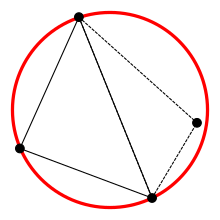
\includegraphics[width=\linewidth]{delaunay_mal}
  \caption{Vértice en el interior de una circunferencia circunscrita. No se cumple la condición de Delaunay}\label{fig:del_mal}
\endminipage\hfill
\minipage{0.32\textwidth}
  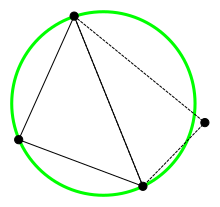
\includegraphics[width=\linewidth]{delaunay_bien}
  \caption{Vértice fuera de una circunferencia circunscrita. Se cumple la condición de Delaunay}\label{fig:del_bien}
\endminipage\hfill
\minipage{0.32\textwidth}%
  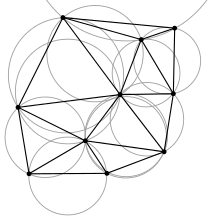
\includegraphics[width=\linewidth]{delaunay_bien_10pts}
  \caption{Triangulación de Delaunay aplicada a 10 puntos. Ninguna  de las circunferencias circunscritas contiene vértices en su interior}\label{fig:del_bien_10pts}
\endminipage
\end{figure}



El origen del nombre de la condición de Delauany se debe al matemático ruso Boris Nikolaevich Delone quien lo ideó en 1934 y tomó la forma francesa de su apellido, "Delaunay" como referencia a sus antecesores franceses.

%https://en.wikipedia.org/wiki/Point_cloud

Por otra parte, una peculiaridad o limitación respecto a las nubes de puntos tiene que ver con que la
información que representan es superficial, es decir, los puntos siempre pertenecen a la superficie del
objeto en cuestión ya que es el lugar donde la luz de los escáneres se llega, rebota y devuelve la
información correspondiente.

Otra desventaja inherente a las nubes de puntos es la interpretación de la información que contienen ya
que se ha explicado que está compuesta de un conjunto de objetos o puntos sin relación entre ellos. Es
aquí donde se requiere intervención del ser humano pues es su cerebro el que puede encontrar la similitud
entre una nube de puntos dada y el objeto o escenario que se supone que representa. Existe software capaz
de encontrar patrones y características para clasificar nubes de puntos pero nunca de forma
completamente fiable (ver aliasing)

El concepto de nube de puntos es eminentemente simple así como versátil y de gran utilidad. Esto se puede apreciar con gran multitud de aplicaciones del concepto de nube de puntos en el mundo real y es que este progreso tecnológico es un gran paso adelante para refinar procesos ya existentes, desde producción a nivel industrial hasta establecer las bases de la navegación de cualquier robot o vehículo.


Ejemplos
hacer nube de puntos simple con visor y poner captura
comparar con cosas como ... (tamaño, numero de puntos, color/no color...)


Se muestran a continuación varios ejemplos de nubes de puntos de diferentes características:

En primer lugar se tiene una sencilla nube de puntos que representa un conejo. Se ha tomado una captura desde uno de todos los posibles puntos de vista que ofrece una visión en 360º.
Un ejemplo algo más elaborado se recoge en la figura 1.5 en la que aparece una nube que representa un lobo. 
Otro ejemplo de mayor complejidad permite observar en la figura 1.6 un escaneo frontal de tres botes de plástico. En este caso, es obvio que las zonas vacías justo detrás de los botes son aquellos lugares donde los rayos de luz emitidos por el sensor no pueden llegar ya que los propios botes los bloquean lo cual sirve para que su superficie quede capturada. Además, se ha incluido un campo de color para cada punto.


\begin{figure}[!htb]
\minipage{0.32\textwidth}
  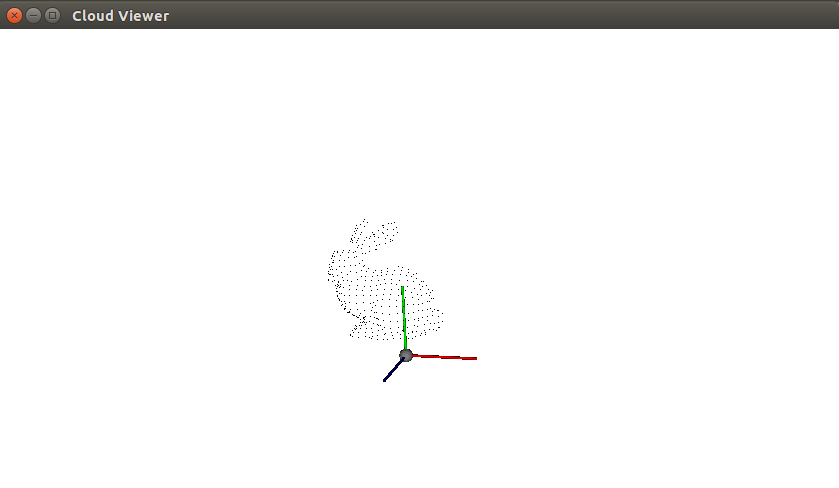
\includegraphics[width=\linewidth]{bunny_simple}
  \caption{Nube de puntos representando un conejo.
  Peso total de la nube: 10.6KB.
  Número total de puntos: 397.}\label{fig:bunny_simple}
\endminipage\hfill
\minipage{0.32\textwidth}
  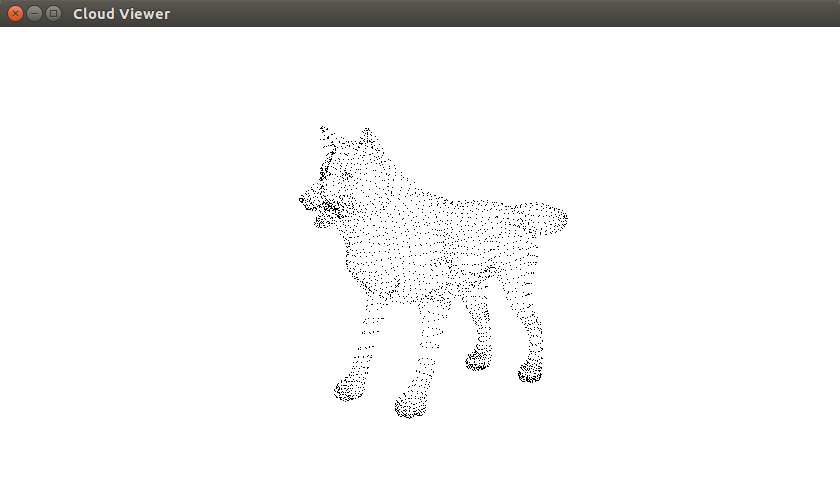
\includegraphics[width=\linewidth]{wolf}
  \caption{Nube de puntos representando un lobo.
  Peso total de la nube: 42.6KB.
  Número total de puntos: 3400.}\label{fig:wolf}
\endminipage\hfill
\minipage{0.32\textwidth}%
  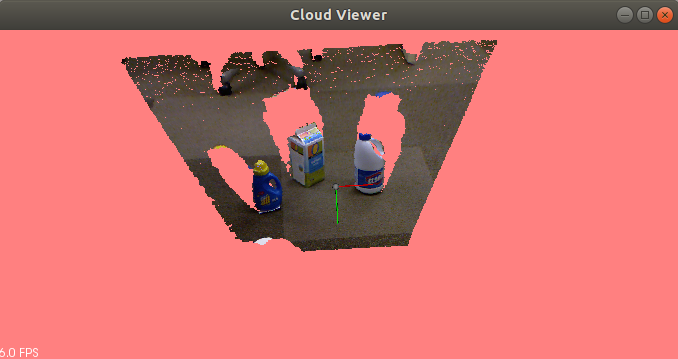
\includegraphics[width=\linewidth]{botes}
  \caption{Nube de puntos representando tres botes.
  Peso total de la nube: 2.43MB.
  Número total de puntos: 307200.}\label{fig:botes}
\endminipage
\end{figure}


%http://www.pointclouds.org/news/2013/01/07/point-cloud-data-sets/
%http://graphics.stanford.edu/data/3Dscanrep/
%http://kos.informatik.uni-osnabrueck.de/3Dscans/
%https://www.cc.gatech.edu/~turk/bunny/bunny.html

Una vez vistos ejemplos de nubes de puntos con la información suficiente para reconocer qué objeto representan sin más ayuda que la de los propios ojos, es momento de subir el nivel de complejidad para dar lugar a nubes de puntos como las que se muestran a continuación:

Se ha visto anteriormente una sencilla representación de un conejo con solamente 397 puntos. El nivel de detalle pude incrementarse a niveles del orden de decenas de miles de pintos tal y como es el caso de la figura 1.6 que representa una figura de arcilla de 7.5 pulgadas de alto con unos 69451 triángulos ya que se ha llevado a cabo la reconstrucción de la superficie. Además, en la figura 1.7 se aprecia el resultado si se añade información sobre color en cada punto.
Como consecuencia de añadir más información (más de 90 veces la cantidad de puntos y el color) se tiene en este caso un peso de 22MB con hasta 35947 puntos.
\begin{figure}[!htb]
\minipage{0.45\textwidth}
  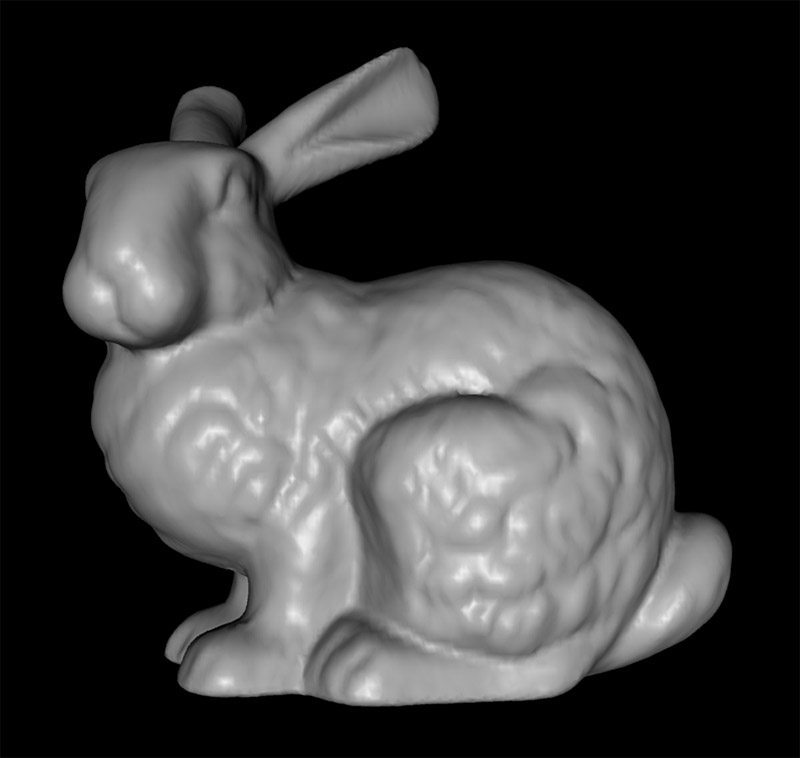
\includegraphics[width=\linewidth]{bunny}
  \caption{Nube de puntos con reconstrucción de superficie representando un conejo sin información de color.}\label{fig:bunny}
\endminipage\hfill
\minipage{0.45\textwidth}
  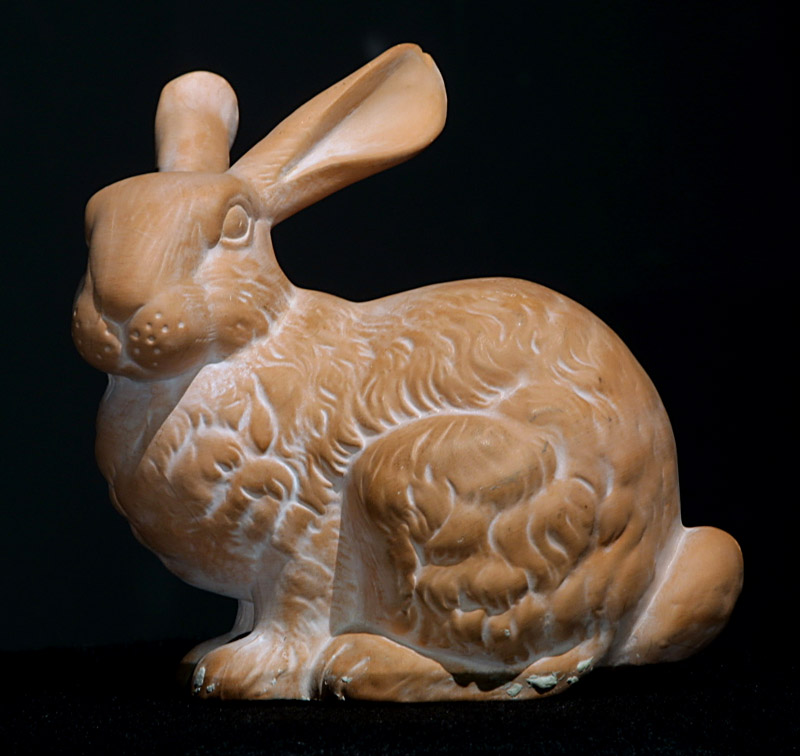
\includegraphics[width=\linewidth]{bunny_colored}
  \caption{Nube de puntos con reconstrucción de superficie representando un conejo con información de color.}\label{fig:bunny_colored}
\endminipage\hfill
\end{figure}
Esta nube de puntos proviene del departamento de computación gráfica de la universidad de Stanford e hicieron falta un total de 10 escaneos con el escaner Cyberware 3030 MS para llegar al resultado final. Para hacerse una idea del tipo de sensor utilizado, se tiene como dato relevante su precio de unos 10000 dólares (ebay) teniendo en cuenta además de que se trata de un sensor antiguo pues el escaneo se produjo en 1993.

Se pueden representar objetos más grandes y con mayor nivel de detalle tal y como se aprecia en la imagen x que representa un dragón construido con madera y resina y con un tamaño de aproximadamente 20cm x 8cm x 9cm.

\begin{figure}
\centering
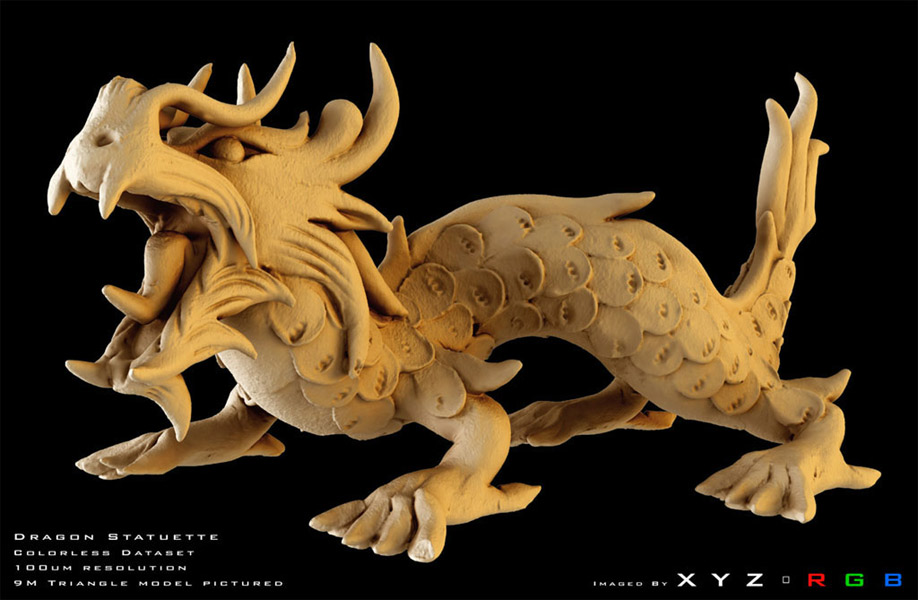
\includegraphics[scale=0.3]{dragon}
\caption{Nube de puntos con reconstrucción de superficie representando una figura de un dragón.}\label{fig:dragon}
\end{figure}

En este caso se han llevado a cabo 18 escaneos con una resolución de 100um o lo que es lo mismo, la separación entre puntos es del orden de 0,1mm. se dispone de un total de 3609455 puntos y 7218906 triángulos lo que implica un peso de 86MB para la nube reconstruida y descomprimida.
La nube de puntos se generó en el mismo laboratorio y con el mismo escaner que se ha mencionado en el caso anterior.

otro objeto de elevada complejidad que ha sido escaneado en las mismas condiciones que el dragón y el conejo es el ángel Lucy. Un total de 47 escaneos dan lugar a un resultado final de 14027932 puntos y 28055742 triángulos y para este caso un peso de 508MB tomando la nube de puntos reconstruida y descomprimida.

\begin{figure}
\centering
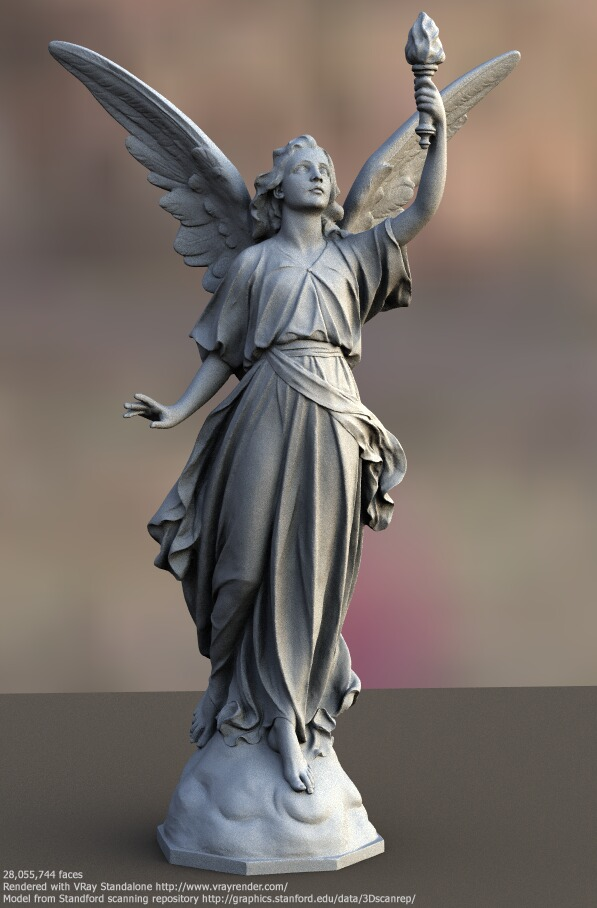
\includegraphics[scale=0.27]{angel_lucy}
\caption{Nube de puntos con reconstrucción de superficie representando una figura de un ángel.}\label{fig:angel_lucy}
\end{figure}

No solamente se pueden representar objetos mediante nubes de puntos sino entornos abiertos o interiores.

Johannes Schauer y Andreas Nüchter de la universidad de Würzburg, Alemania, tomaron la siguiente nube de puntos del mercado en la ciudad de Würzburg.
El escaner utilizado en el este caso es el Riegl VZ-400 y con un total de 6 escaneos se han conseguido 86585411 puntos conteniendo cada uno de ellos información sobre la reflectancia de la luz del sensor lo que se representa con puntos de diferente claridad ya que no hay información sobre color. Obviamente, un entorno exterior contiene mucha más información que un simple objeto por lo que esta nube de puntos tiene un peso de 5117MB descomprimida.

Cabe destacar que el sensor utilizado es bastante más potente que el anterior mencionado y tiene un precio de unos 80000 dólares.

\begin{figure}
\centering
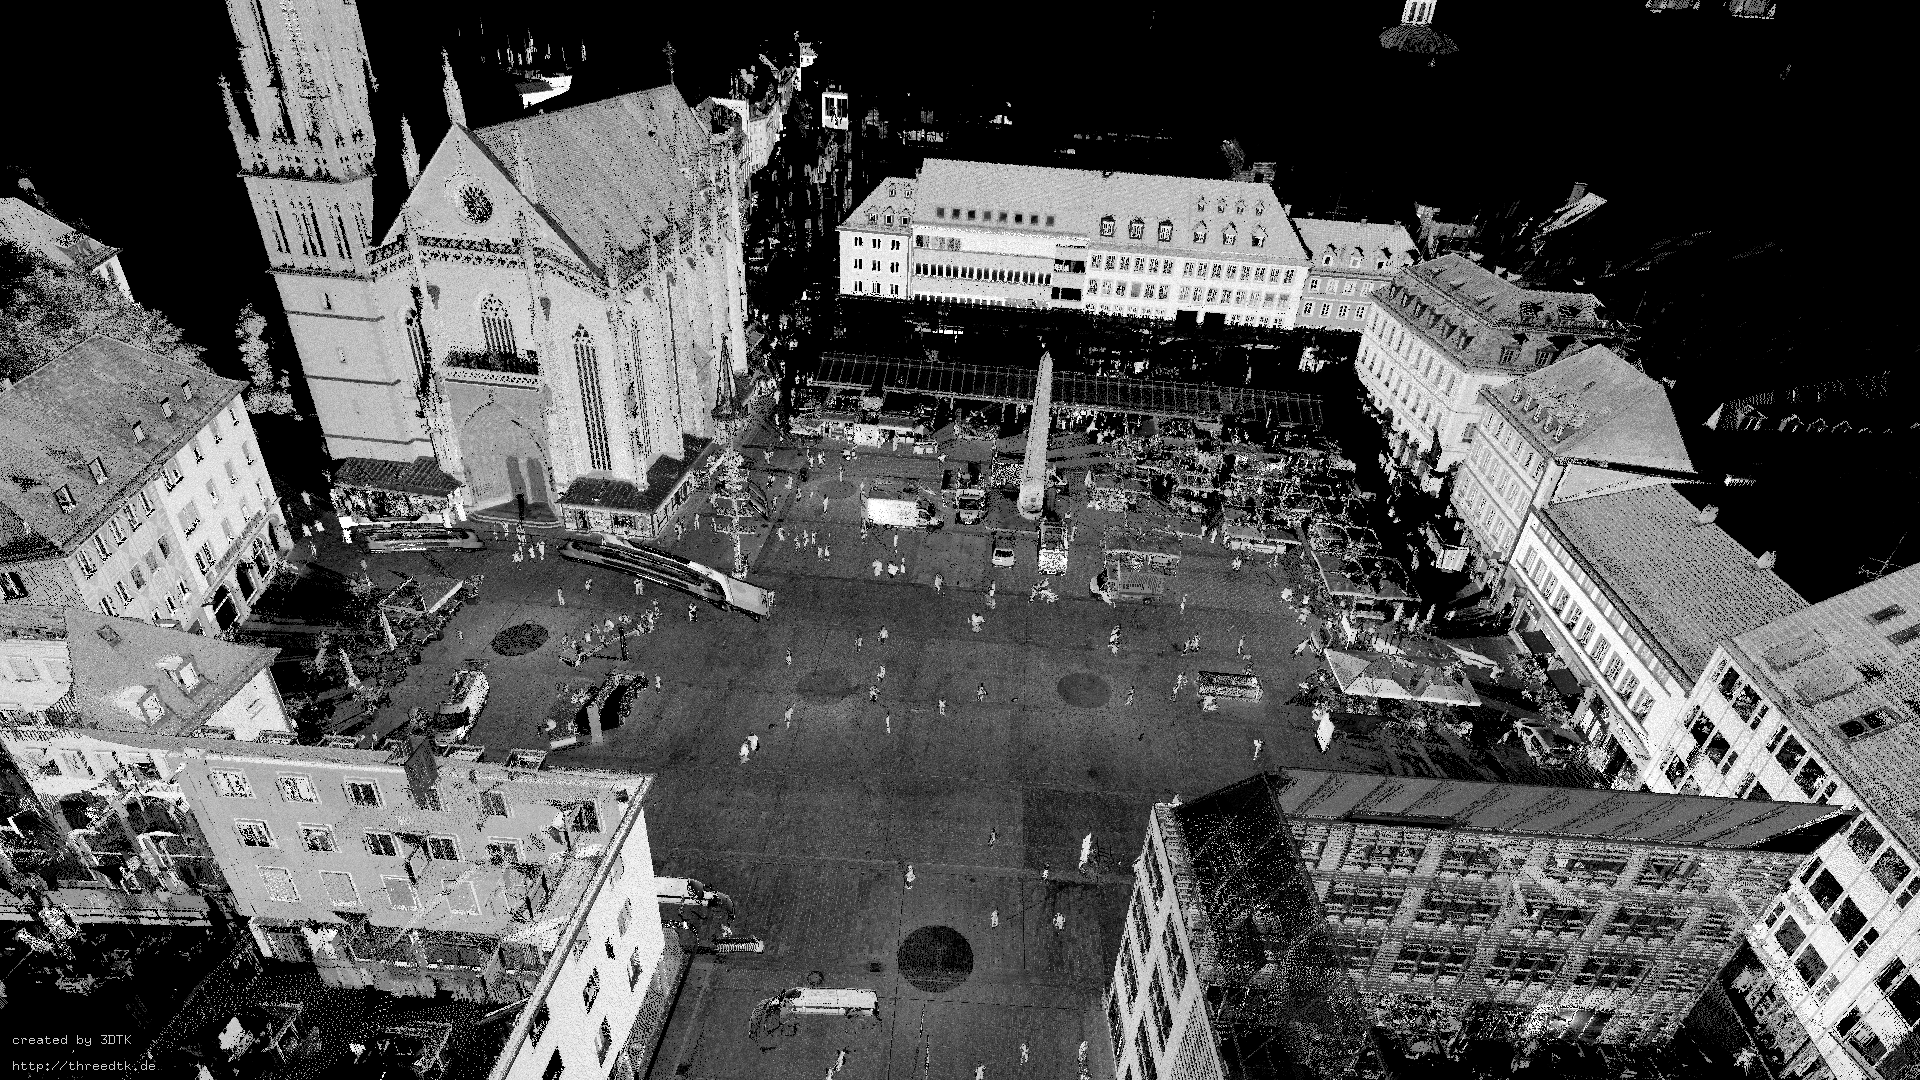
\includegraphics[scale=0.17]{wue_city2}
\caption{Nube de puntos con información de reflectancia de la luz que representa un mercado en Würzburg, Alemania.}\label{fig:wue_city}
\end{figure}

Por último, Dorit Borrmann obtuvo una nube de puntos que representa el interior del laboratorio de automática en la universidad de Jacobs, Bremen. Se pueden apreciar diferentes tipos de puntos para cada sección de la imagen ya que el sensor láser Riegl VZ-400 se encarga de representar información térmica y de profundidad mientras que las cámaras Optris PI IR y Logitech QuickCam 9000 Pro muestran información relacionada con el color.

\begin{figure}
\centering
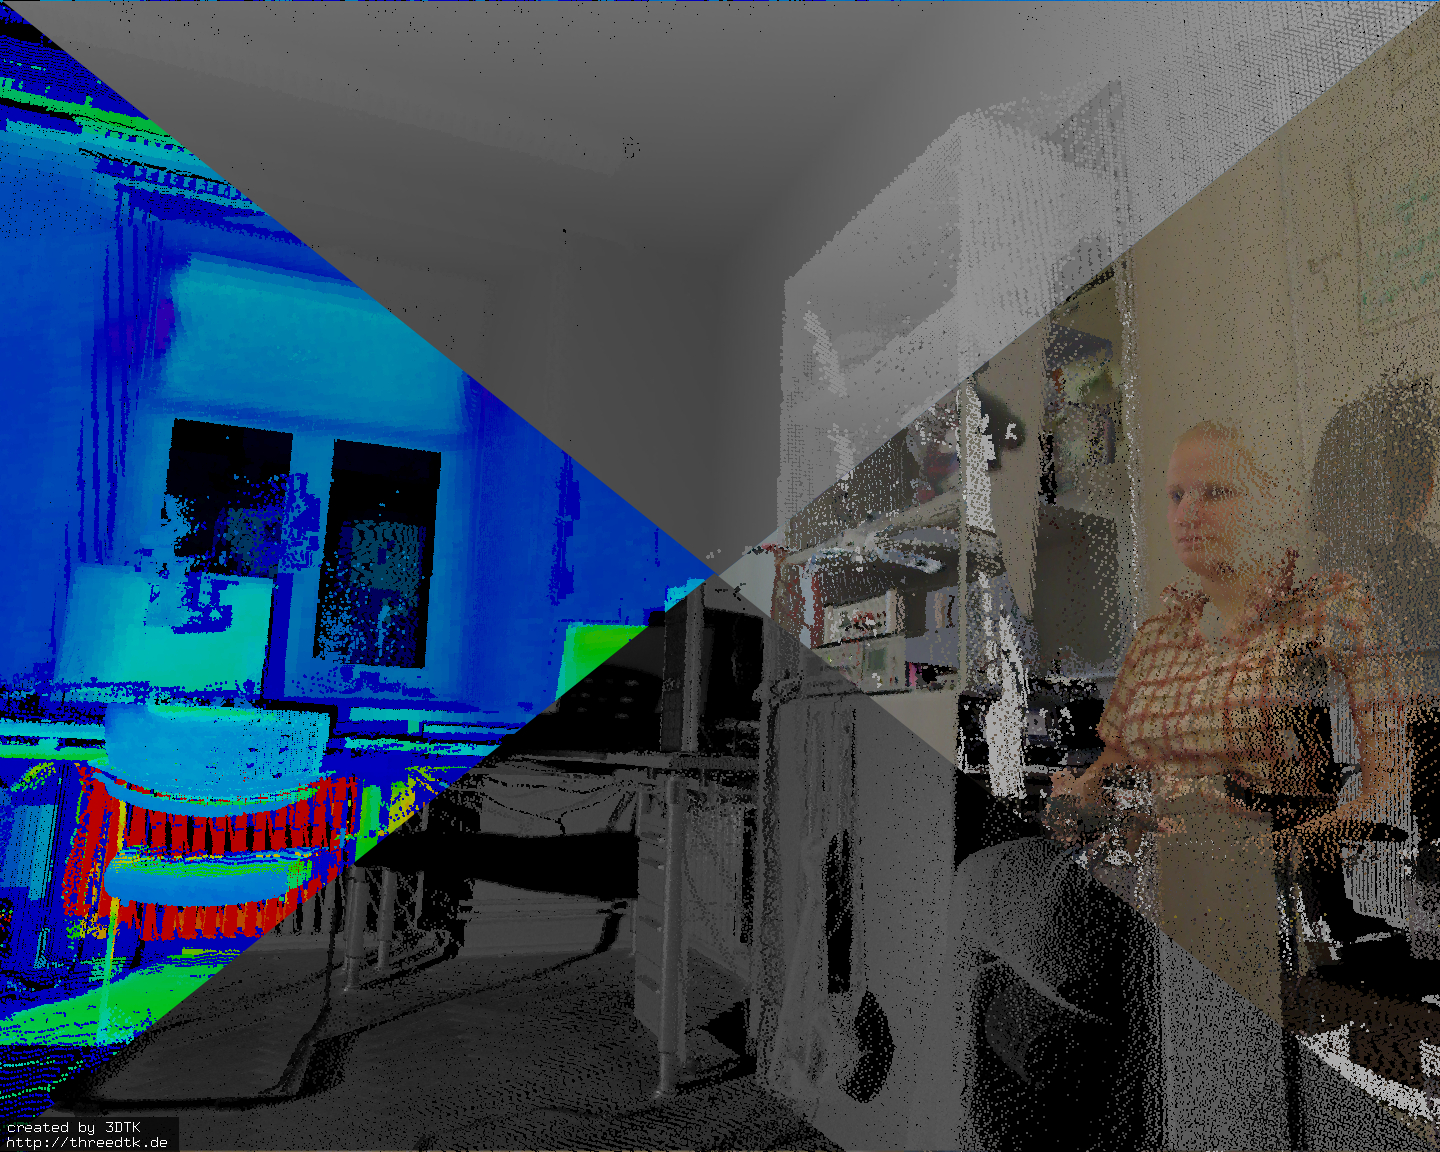
\includegraphics[scale=0.17]{joinedmodel}
\caption{Unión de cuatro nubes de puntos con información térmica, de color y reflectancia de la luz representando un entorno cerrado.}\label{fig:joined_model}
\end{figure}

Se hicieron un total de 9 escaneos en 40º cada uno lo que permite disponer de una imagen en 360º (la imagen mostrada es uno de los escaneos)




\section{Adquisición de información: Sensores y evolución}

La adquisición y almacenamiento de información es el primer paso para comenzar a trabajar con una nube de puntos. A pesar de tratarse de información relativamente sencilla como coordenadas respecto a un sistema de referencia, color y reflectividad, hay que tomar dicha información para miles o incluso millones de puntos tal y como se ha visto en ejemplos mostrados anteriormente como en el caso del ángel Lucy (figura ). Por lo tanto, el factor limitante del sensor en cuestión radica en cuánta y cuan variada información es capaz de percibir y almacenar.

En los últimos veinte años, se han hecho grandes progresos en lo que a sensores e refiere ya que actualmente se usan de sofisticadas cámaras y escaneres láser y se han dejado atrás los sensores basados en sonar o infrarrojos los cuales proporcionan a penas unos bytes de información sobre el entorno u objeto que tratan de representar.


Centrándose en los sensores láser, la adquisición de información cobra sentido cuando se tienen en cuenta la desviación de rayos de luz ya sea visible o infrarroja, por ejemplo.




 Para poder llevar a cabo el escaneo de objetos tridimensionales así como entornos, el escaneo laser o también conocido como lidar (light detection and ranging pero originalmente se conocía por la union de light and radar), 
es un procedimiento que se originó a principios de la década de los sesenta tras la invención del láser y permite medir distancias a un objetivo iluminándolo con pulsos láser y estudiando los tiempos de retorno y longitudes de onda de estos pulsos al rebotar y ser captados por un sensor conocido como rangefinder. 

De este modo, al ser capaz de medir la distancia que hay desde el punto de emisión de los rayos de luz hasta la superficie en la que rebotan, el sensor puede detectar rápidamente formas definidas de objetos, edificios o paisajes considerando en conjunto de puntos detectados.


Por lo general, hay dos tipos de lidar:
método coherente e incoherente o también conocido como detección de energía directa.
El método incoherente mide cambios en la amplitud de la onda emitida pues al rebotar e interactuar con el ambiente su nivel de energía varía.

imagen cambio amplitud

El método coherente es más apropiado para medir diferencias en la frecuencia de la onda y utiliza (Optical heterodyne detection) lo que le permite operar a potencias mucho más bajas a costa de utilizar un equipamiento mucho más complejo (more complex transceiver requirements)

imagen cambio fase


En ambos modelos se pueden usar dos tipos diferentes de pulsos: micropulsos y sistemas de alta energía.
los micropulsos surgen de la elevada capacidad computacional de las computadoras actuales. Esto deriva en un láser de baja potencia (del orden del microjulio) que es clasificado como seguro al ojo permitiéndose su uso bajo escasas medidas de precaución 

Por otra parte, los sistemas de alta energía, requieren medidas de seguridad más estrictas y se usan principalmente para fines de investigación atmosférica pues permite tomar medidas como la altura, número de capas y densidad de las nubes, propiedades de las partículas en las nubes, temperatura, presión, concentración de gases, o humedad.



Para cada pulso de luz emitido se detecta un punto en concreto lo que hace pensar que para poder crear nubes con millones de puntos la velocidad de generación de los pulsos ha de ser elevada. En el caso de lidar se pueden emitir hasta 150000 pulsos en un segundo.

Pero ¿Cómo se pueden medir distancias utilizando luz? el concepto entorno al que el escaner laser gira es el tiempo de vuelo. Esto quiere decir que se utiliza un dispositivo (range finder) capaz de medir con precisión el tiempo que transcurre desde que se emite un pulso de luz hasta que vuelve otra vez al mismo tras rebotar sobre el objeto que desea detectarse. Considerando entonces que la velocidad de la luz es una constante conocida, c, la distancia del escaner a un punto en concreto donde rebota un determinado pulso de luz puede determinarse como:

ecuacion d= c*t/2

Nótese que c*t es la distancia que hay entre el escaner y el objeto duplicada ya que t es el tiempo total desde la emisión del pulso de luz hasta la recepción. Por tanto, tomando la mitad del tiempo total de vuelo se obtiene la medida deseada que es la distancia del escaner al objeto.

Retomando la idea de que la velocidad de la luz es una constante, la única variable en el cálculo de la distancia es el tiempo de vuelo. Téngase por ejemplo una distancia de 30cm desde el sensor hasta el objeto que desea capturarse.Esto implica que la resolución del reloj integrado en el sensor ha de ser cuanto menos elevada:

%0,3m/3*10^8=1ns=0,000000001s, en ese tiempo...

Se ha desvelado de esta forma una desventaja del concepto de tiempo de vuelo, se necesita equipamiento muy preciso y fiable lo que se traduce en complejidad y elevadas inversiones económicas.

Pero dando la vuelta a esta desventaja, es decir, cuando se trata de escanear objetos en la lejanía como puede ser un edificio o paisaje,la resolución requerida por parte del reloj se reduce dando así medidas más fiables. Además, considerando de nuevo la velocidad de la luz como una constante, no importa la distancia a la que se encuentre el objeto salvo por cuestiones de difracción y absorción del pulso de luz en el ambiente, por ejemplo , por la presencia de humedad.

Una aplicación muy extendida del lidar es el reconocimiento de terreno. Para ello se integra el sensor en una aeronave y se capturan los puntos correspondientes al terreno sobrevolado. Esta aplicación es útil para generar modelos digitales de elevación.



 

Este método combina precisión y versatilidad ya que puede valerse de luz visible, infrarroja o ultravioleta para lanzarla contra objetivos de diversos tipos de materiales como metal, cerámica, aerosoles, terreno (rocas y tierra) e incluso se puede llegar al nivel molecular. 
 


imagen

Sin embargo no se realiza un único escaneo ya que el propio concepto implica que el objeto bloquea los rayos de luz por lo que la cara frontal, de la que sí se obtiene información, impide a la luz llegar a la cara posterior. El factor clave es entonces el hecho de que estos rayos de luz puedan llegar a toda la superficie del objeto que se quiere analizar, es decir, accesibilidad física del sensor.
De este modo, independientemente del sensor o método que se utilice, es imposible recolectar
información sobre superficies no visibles o lo que es lo mismo, con un solo escaneo.


imagen 


Como consecuencia, es necesario llevar a cabo varios escaneos desde diferentes puntos de vista y
ponerlos en conjunto conociendo con precisión la posición del sensor en cada escaneo.




En cuanto a los componentes necesarios para cualquier sistema lidar 

Aplicaciones/dispositivos:

\textit{mencionar y describir alguna aplicación relevante ejemplo: Velodyne spinning LIDAR https://en.wikipedia.org/wiki/Lidar}




%https://upload.wikimedia.org/wikipedia/commons/c/c0/LIDAR-scanned-SICK-LMS-animation.gif
%https://www.engineering.com/AdvancedManufacturing/ArticleID/12390/Quality-Basics-How-Does-3D-Laser-Scanning-Work.aspx
%https://en.wikipedia.org/wiki/Laser_scanning
%http://www.2grobotics.com/wp-content/uploads/2017/03/sonarvslaser.pdf
%http://www.lidar-uk.com/how-lidar-works/

Disponer de complejas, fiables y robustas representaciones del mundo real tiene no es tan sencillo como pueda parecer puesto que estos sensores suelen tener un precio prohibitivo para la mayoría de los interesados ya sean particulares o incluso empresas con un poder adquisitivo considerable. Sin embargo, las tornas han cambiado desde que han aparecido en el mercado ciertos sensores 3D como por ejemplo el sensor Kinect de la consola Xbox360 de Microsoft. Este sensor está basado en la tecnología PrimeSense y aunque puede trabajar con nubes de puntos en tiempo real e imágenes en 2D su precio no supera los 150\$. De este modo se ha producido un gran paso adelante en cuanto a los impedimentos relacionados con la adquisición, mantenimiento y delicadeza del hardware que traduce el mundo real a nubes de puntos.

\section{Procesamiento software de información }
\section{objetivos}
Una vez estudiado el hardware necesario se precisa ahora de un mecanismo para trabajar con la inmensa cantidad de información que aportan los sensores. 

El software existente para dicha tarea es diverso y no siempre gratuito. Como ejemplos se tienen:
\begin{list}{-}
\item 3DF Zephyr
\item RealityCapture
\item Agisoft Photoscan
\item Point cloud tool

\textit{describir brevemente y mencionar impedimentos de precio, limitaciones etc
}
\end{list}




Es aquí donde entra en juego una librería de código abierto llamada PCL (insertar imagen-web) siglas que en inglés representan Point Cloud Library, traducible como librería de nubes de puntos.

\textit{Definir qué es pcl, historia, extensión
http://pointclouds.org/
paper: 3D is here}


\section{Descripción de herramientas}
\subsection{Herramientas hardware}
\subsection{Herramientas software}


Generar un programa capaz de obtener keypoints a partir de una nube de puntos
Croscompilar usando las herramientas de xilinx 
Enviar ejecutable a la placa y ejecutar el programa
(optimización)

